\ifthenelse{\boolean{english}}{
	\chapter{Introduction \& Scope}
}{
	\chapter{Einleitung \& Aufgabenstellung}
}
\label{cha:einleitung}

\section{Unterkapitel der Einleitung}
\label{sec:unterkapitel_der_einleitung}

Man kann auch auf andere Kapitel, wie z.~B. auf Kapitel~\ref{cha:ergebnis} verweisen oder man verweist auf einen Abschnitt, z.~B. auf den Abschnitt~\ref{sec:unterkapitel_der_einleitung}.

\subsection{Unter Unterkapitel der Einleitung}
\label{sec:unter_unterkapitel_der_einleitung}

Die Abk"urzung APDL \nmA[APDL]{APDL}{ANSYS Parametric Design Language} wird im Abk"urzungsverzeichnis erl"autert. Das $F_D$ \nmD[F]{$F$}{Kraft}{\si{N}} \nmI[D]{D}{Druck} steht f"ur die Druckkraft und wird auch im Symbolverzeichnis gef"uhrt. Das $\alpha$ \nmG[alpha]{$\alpha$}{Winkel}{\si{rad}} steht f"ur die Beschleunigung und ist auch im Symbolverzeichnis gef"uhrt.

\subsubsection{Unter unter Unterkapitel der Einleitung}
\label{sec:unter_unter_unterkapitel_der_einleitung}


\figurename~\ref{fig:testbild} zeigt ein Testbild. Dabei dient der Name \emph{fig\:testbild} zum Referenzieren auf die \figurename~\ref{fig:testbild} mit fig\_hol = figure\_hollaus, um Mehrfachbenennungen von Bildern zu vermeiden (vor allem wenn mehrere Studenten an einem Dokument arbeiten). Hinsichtlich der Aufl"osung der Bilder ist es am besten die Bilder als Vektorgrafiken z.B. unter \emph{.eps} abzuspeichern. So hat man immer die beste Qualität der Bilder.

% beginn Kommentar
\begin{comment}

Dieser Text wird nicht Angezeigt.

% ende des Kommentars
\end{comment}

\begin{figure}[H]
\centering
\begin{tikzpicture}
	\node at (0,0) {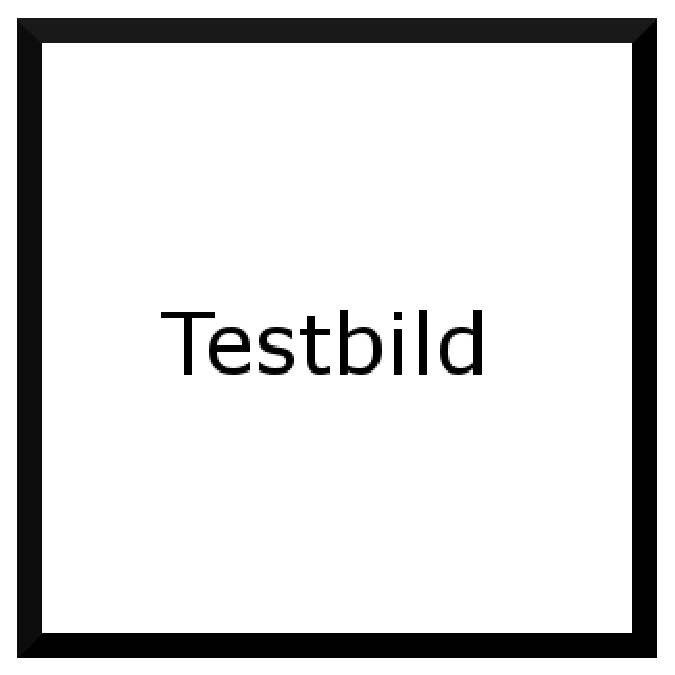
\includegraphics[width=0.33\bildbreite]{bilder/testbild}};
\end{tikzpicture}
\caption[Kurze Abbildungsbeschreibung f"ur das Abbildungsverzeichnis]{Abbildungsbeschreibung f"ur das Testbild\atlbe}
\label{fig:testbild}
\end{figure}

%\begin{figure}[H]\centering
%\includegraphics[scale=0.5]{Bilder/Stromregler.png}
%\caption{Versuchsschaltung Stromregler}
%\label{abb:stromregler}
%\end{figure

\tablename~\ref{tab:testtabelle} zeigt eine Testtabelle. In TexMaker l"a{\ss}t sich relativ schnell und komfortabel eine Tabelle mittels dem eingebauten Tabellen-Assistenten erstellen (zu finden unter \emph{Assistent}$\rightarrow$\emph{Tabellen-Assistent}).

\begin{table}[H]
\caption[Kurze Bennennung der Tabelle mit den technischen Daten f"ur das Tabellenverzeichnis]{Technische Daten\atlbe}
\centering
\begin{tabular}{cc}
\toprule
\multicolumn{2}{c}{\textbf{Testwerte}}\\
\midrule
Kraft & $\SI{1}{kN}$\\
L"ange & $\SI{1}{m}$\\
\bottomrule
\end{tabular}
\label{tab:testtabelle}
\end{table}

Es kann auch eine Schaltung \figurename~\ref{fig:schaltung} in Latex gezeichnet werden.

\begin{figure}[H]
\centering
\begin{circuitikz}[scale=1]\draw
 (0,8) -- (2,8)
 (0,10) node [left] {$U_{IN}$} to [switch, l=$S_1$, o-*] (2,10)
 to [L, l=$L$, *-o] (4,10) to [short, *-o] (5,10) node [right] {$U_{OUT}$}
 (4,10) to [capacitor, l_=$C$, -*] (4,8) node[rground]{}
 (2,8) to [opening switch, l=$S_2$, *-*] (2,10)
 (0,8) node [left] {$GND$} to [short, o-o] (5,8) node [right] {$GND$}
;\end{circuitikz}
\caption[Aufbau buck converter]{Aufbau buck converter\atlbe}
\label{fig:schaltung}
\end{figure}